\section*{Materials and Methods}  % temporary section name

Statistical alignment is typically performed using pairwise hidden Markov models (pair-HMMs), which have the ability to rigorously model molecular sequence evolution \parencite{bradley2007transducers}.
Pair-HMMs are computational machines with two output tapes that contain a finite number of states typically labeled match, insert, and delete that emit symbols (nucleotides or amino acids) to one or both tapes.
Each tape represents a sequence and a path through a pair-HMM is a possible pairwise alignment.
Conceptually, these machines generate two sequences ($X$ and $Y$) from an unknown ancestor and can calculate the probability that two sequences are related, represented by $P(X, Y)$ \parencite{yoon_2009_hmm}.

A limitation of pair-HMMs is the ability to only model the evolution of two related sequences from an unknown ancestor.
Finite-state transducers (FSTs) have similar benefits to pair-HMMs with the additional feature to generate a descendant sequence given an ancestral one.
FSTs consume symbols from an input tape and emit symbols to an output tape.
Properly weighted, an FST can calculate the probability that a descendant sequence $Y$ evolved from an ancestor sequence $X$, represented by $P(Y | X)$.
Furthermore, well-established algorithms for combining FSTs in different ways allow the design of complex models by combining simpler FSTs \parencite{bradley2007transducers}.
A powerful and versatile algorithm for comparative sequence analysis is composition, which consists of sending the output of one FST into the input of a second FST.
The model implemented in COATi is designed by composing smaller FSTs, each representing a specific process.

Genomes for model organisms are often of high quality after being refined over many iterations and having their coding sequences meticulously curated.
On the contrary, non-model organisms typically have lower-quality genomes that have been only partially curated.
Low-quality genomes often lack the amount of sequencing data needed to fix artifacts, including missing exons, erroneous mutations, and indels \parencite{jackman2018tigmint}.
FSTs and their powerful methods provide a well-suited framework to statistically align a sequence from a non-model organism against a sequence from a model organism.

COATi implements the pairwise alignment of a low-quality sequence (descendant)  against a high-quality sequence (ancestor) as a path through the Evolution FST (Fig. \ref{fig:evolution-fst}), based on existing transducers (e.g. \cite{holmes2001evolutionary}).
This FST is the result of composing a substitution FST that encodes a codon model (Fig. \ref{fig:evolution-fst}-a) and an indel FST that models insertions and deletions, including frameshifts (Fig. \ref{fig:evolution-fst}-b).
A key innovation of this FST with respect to others is the combination of a codon substitution model with a nucleotide-based geometric indel model that allows gaps to occur at any position.

Composing both sequences with the Evolution FST results in the transducer of all possible alignments.
Any path through this FST represents a pairwise alignment, while the shortest path corresponds to the best alignment.
All FST operations in COATi, including model development, composition, search for the shortest path, and other optimization algorithms, are performed using the C++ openFST library \parencite{allauzen2007openfst}.

\begin{figure}[h!]
\begin{framed}
\centering
    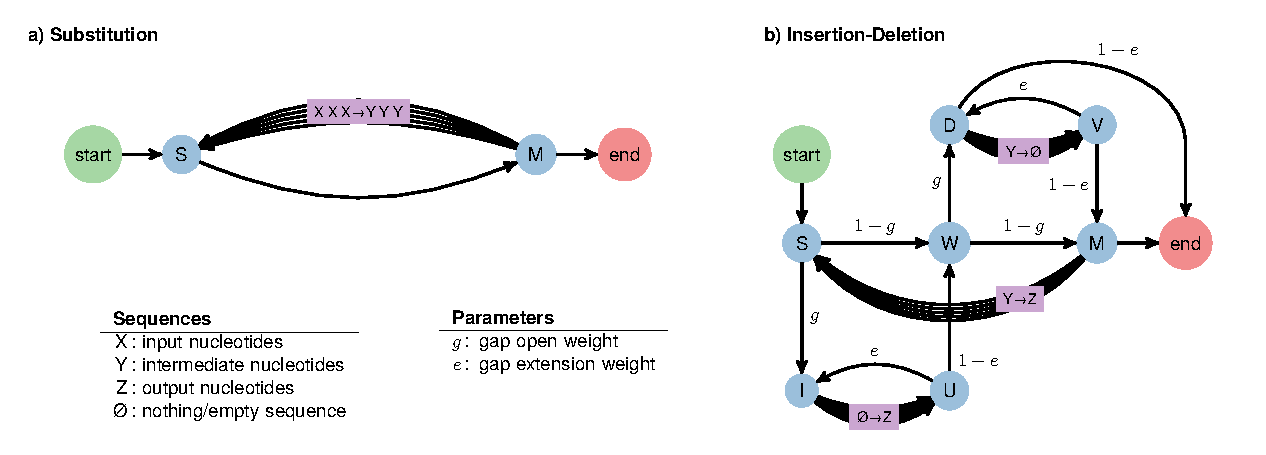
\includegraphics[width=\textwidth]{fig-evolution-fst.pdf}
    \caption{The Evolution FST is assembled by composing a substitution FST and
    an indel FST. Each node represents a state in an FST while arcs display
    possible transitions between states (and their weights). (a) The
    substitution FST encodes a 61x64 codon substitution model with $61\cdot 64$ arcs
    from M to S. (b) The indel FST allows for insertions (I to U) and deletions
    (D to V). Contiguous insertions and deletions are always arranged for
    insertions to precede deletions to limit equivalent alignments.}
    \label{fig:evolution-fst}
\end{framed}
\end{figure}

Codon substitution models are uncommon in sequence aligners, despite their extensive use in phylogenetics.
COATi implements the Muse and Gaut (1994) codon model (codon-triplet-mg) and the Empirical Codon Model \parencite{kosiol_ECM_2007} (codon-triplet-ecm).
It also lets the user provide a codon substitution matrix.
The default FST model (codon-triplet-mg) does not allow substitutions from stop codons, although it supports mutations to (early) stop codons under the assumption that these are artifacts common in low-quality data.

COATi also features a marginal substitution model with probability matrix

\[P'_{ijp} = \mathlarger{\mathlarger{\sum}}_{cod} \thickspace \begin{cases}
P(i \thinspace | \thinspace cod) \enspace \text{if} \enspace cod_p = j\\
0 \enspace \text{otherwise}
\end{cases} \]

Where $P'_{ijp}$ represents the probability that codon $i$ from the ancestor
sequence changes to nucleotide $j$ of the descendant sequence at position $p$
$\in \{0, 1, 2\}$ of the reading frame.
$P$ is the substitution probability matrix Muse and Gaut or the Empirical Codon Model, resulting in the marginal models codon-marginal-mg (default model) and codon-marginal-ecm.
These models emphasize the position where the substitution in a codon occurs, help restrict the effects of low-quality data in the descendant sequence, and allow more than one substitution per codon.
In combination with the indel model, alignment using the marginal model is implemented using dynamic programming.
